\documentclass{article}
\usepackage[left=3cm,right=3cm,
    top=2cm,bottom=2cm,bindingoffset=0cm]{geometry}
\usepackage{graphicx} % Required for inserting images

\usepackage[english, russian]{babel}
\usepackage[T2A]{fontenc}			% кодировка
\usepackage[utf8]{inputenc}			% кодировка исходного текста
\usepackage{amsmath,amsfonts,amssymb,amsthm,mathtools}

\title{\textbf{Лабораторная работа 1.2.3.} \linebreak
ОПРЕДЕЛЕНИЕ МОМЕНТОВ ИНЕРЦИИ ТВЕРДЫХ ТЕЛ С ПОМОЩЬЮ ТРИФИЛЯРНОГО ПОДВЕСА}
\author{Попова Софья Б04-401}
\date{November 2024}

\begin{document}

\maketitle

\section*{Цель работы}
Измерение момента инерции ряда тел и сравнение результатов с рассчетами по теоретическим формулам; проверка аддитивности моментов инерции и справедливости формулы Гюйгенса-Штейнера

\section*{Оборудование}
Трифилярный подвес, секундомер, счетчик числа колебаний, набор исследуемых тел (диск, полый цилиндр, две половины диска) 

\section*{Теоретическая часть}
Момент инерции твердого тела относительно неподвижной оси вычисляется по формуле: 
\begin{equation}
    I=\int_{}^{}r^2dm
\end{equation}

\noindent
Трифилярный подвес состоит из укрепленной на некоторой высоте неподвижной платформе $P$ и подвешенной к ней на трех симмметрично расположенных нитях $AA', BB', CC'$ вращающейся платформы $P'$. Для экспериментального измерения момента инерции нижнюю платформу закручивают на определенный угол вокруг неподвижной оси и при возвращении к положению равновесия вызываются крутильные колебания. Если пренебречь потерями энергии на трение, то уравнение сохранения энергии можно записать так: 
\begin{equation}
    \frac{I\dot{\varphi}^2}{2} + mg(z_0 - z) = E
\end{equation}
Дважды дифференцируя по времени, после сокращений, получаем:	
\begin{equation}
	I\ddot{\phi}^2 + mg\frac{Rr}{z_{0}}\phi = 0 
\end{equation}
Решая уравнение относительно $\phi$, получаем:
\begin{equation}
	\phi = \phi_{0}\sin\left(\sqrt{\frac{mgRr}{Iz_{0}}}t + \theta\right)
\end{equation}

\noindent
Период крутильных колебний системы равен:
\begin{equation}
    T = 2\pi \sqrt{\frac{Iz_0}{mgRr}}
\end{equation}
Тогда формула для вычисления момента инерции:
\begin{equation}
    I = \frac{mgRrT^2}{4\pi^2z_0}  \ \ \ \text{или}  \ \ \ I=kmT^2
\end{equation}
где $k = \frac{gRr}{4\pi^2z_0}$ - постоянная

\section*{Экспериментальная часть}
\subsection*{Определение константы}
Параметры установки:
\begin{itemize}
    \item $r = 30,5 \pm 0,3$ мм
    \item $R = 114,1 \pm 0,5$ мм
    \item $m= 1,0048 \pm 0,0005$ кг
    \item $z_0 = 2175 \pm 0,5$ мм
\end{itemize}

\noindent
По этим значением получена $k \approx 0,397$ $(\sigma_k = \sqrt{(\frac{\sigma_R}{R})^2 + (\frac{\sigma_r}{r})^2 + (\frac{\sigma_{z_0}}{z_0})^2} = 0,016)$

\subsection*{Определение момента инерции ненагруженной платформы}
Для определения момента инерции вычислим период колебаний пустой платформы. Измерения указаны в таблице($N$ - количество колебаний, $t$ - время $N$ колебаний, $T$ - период колебаний):
\begin{table}[h]
    \centering
    \begin{tabular}{|c|c|c|}
    \hline
        N  & t(c) & T_0(c) \\
    \hline
        10 & 43,67 & 4,367 \\
        10 & 43,82 & 4,382 \\
        10 & 43,68 & 4,368 \\
        10 & 43,36 & 4,336 \\
        10 & 43,73 & 4,373 \\
    \hline
    \end{tabular}
    \label{tab:my_label}
\end{table}

$T_{0(\text{сред})} = \frac{4,367 + 4,382 + 4,368 + 4,336 + 4,373}{5} = 4,36$ секунды

\

\noindent
Момент инерции вычисялется по формуле (6):

\

$I_0 = 0,3971 \cdot 1,0048  \cdot 4,365^2 = 7,6$ кг·м²

\ 

$\sigma_{I_0} = \sqrt{(\frac{\sigma_k}{k}) + (\frac{\sigma_m}{m}) + 2 \cdot (\frac{\sigma_T}{T})}  = \sqrt{(\frac{0,0166}{0,3971})^2 + (\frac{0,0005}{1,0048})^2 + 2 \cdot (\frac{0,017}{4,3652})^2} = 0,042$


\subsection*{Проверка аддитивности моментов инерции}

\noindent
Для проверки аддитивности моментов инерции измерены моменты инерции двух тел: полого цилиндра и диска, и их суммарный момент инерции. Результаты измерений указаны в таблице ($N$ - количество колебаний, $t$ - время $N$ колебаний, $T$ - период колебаний):

\begin{table}[h]
    \centering
    \begin{tabular}{|c|c|c|c|c|c|c|c|c|}
    \hline
        \multicolumn{3}{|c|}{Полый цилиндр} & \multicolumn{3}{|c|}{Диск} & \multicolumn{3}{|c|}{Два тела}\\
    \hline
        N & t(c) & T_1(c) & N & t(c) & T_2(c)  & N & t(c) & T_{1+2}(c) \\
    \hline
        10 & 42,16 & 4,216 & 10 & 39,22 & 3,922 & 10 & 39,57 & 3,957 \\
        10 & 42,19 & 4,219 & 10 & 39,17 & 3,917 & 10 & 39,53 & 3,953 \\
        10 & 42,54 & 4,254 & 10 & 39,14 & 3,914 & 10 & 39,51 & 3,951 \\
        10 & 42,13 & 4,213 & 10 & 39,24 & 3,924 & 10 & 39,61 & 3,961 \\
        10 & 42,20 & 4,22  & 10 & 39,17 & 3,917 & 10 & 39,59 & 3,959 \\
    \hline
    \end{tabular}
\end{table}

\newpage
\noindent
Характеристики тел:

\noindent
Полый цилиндр
\begin{itemize}
    \item $m = 820,7 \pm 0,5$ г
    \item $r_{\text{внеш}} = 8,3 \pm 0,05$ см 
    \item $r_{\text{внутр}} = 7,9 \pm 0,05$ см
\end{itemize}
Диск
\begin{itemize}
    \item $m = 585,3 \pm 0,5$ г
    \item $r = 8,55 \pm 0,05$ см
\end{itemize}
Цилиндр + диск
\begin{itemize}
    \item $m = 1406 \pm 0,5$ г
\end{itemize}

\

\noindent
$T_{1(\text{сред})} \approx 4,22$ с

\noindent
$T_{2(\text{сред})} \approx 3,92$ с

\noindent
$T_{1+2(\text{сред})} \approx 3,96$ с

\

\noindent
Момент инерции вычисялется по формуле (6):

\noindent
(здесь к массе тел прибавляется масса платформы, $I_{1}$ - момент инерции цилиндра и платформы,  $I_{2}$ - диска и платформы, $I_{1+2}$ - диска, цилиндра и платформы)

\noindent
$I_{1} \approx 12,91$ кг·м²

\noindent
$I_{2} \approx 9,7$ кг·м²

\noindent
$I_{1+2} \approx 15,01$ кг·м²

\

\noindent
Если аддитивность момента инерции выполняется, то $(I_1-I_0) + (I_2-I_0) = I_{1+2}-I_0$:

\noindent
$(12,91-7,6) + (9,7-7,6) = 7,41 = 15,01-7,6$ - выражение верно. В связи с округлением до сотых, результаты совпали точно, что может говорить о достаточно высокой точности такого способа доказательства аддитивности, но не следует делать вывод о том, что показания будут идеально точны, так как значения могут расходиться при менее грубом округлении. 

\noindent
В таком случае можно вычислить полученные экспериментально значения:

$I_\text{ц} = I_1-I_0 = 12,91 - 7,6 = 5,31$ кг·м²

$I_\text{д} = I_2-I_0 = 9,7 - 7,6 = 2,1$ кг·м²

\

\noindent
Теперь сравним полученные нами моменты инерциии для тел, и их теоретические значения. Для цилиндра момент инерции вычисляется так же как и для диска: $I_\text{ц} = \frac{1}{2}m_\text{ц}R_\text{ц}^2$. Радиус данного диска $R_\text{д} = 8,55$ см, тогда $I_\text{д} = 2,139$ кг·м²$\cdot 10^{-3}$, что подтверждает экспериментальное значение.

\noindent    
Для кольца же: $I_\text{к} = m_\text{к}R_\text{к}^2$. Так как данное кольцо не идеально тонко, то $R_\text{к} = \frac{r_\text{внутр} + r_\text{внеш}}{2}$, тогда $R_\text{к} = 8,1 \text{ см}$. Получаем, что $I_\text{к} = 5,384$ кг·м²$\cdot 10^{-3}$, что тоже примерно совпадает с полученным экспериментально значением.

\noindent
Разница между экспериментально и теоретически полученными значениями: $\frac{2,139-2,1}{2,139} \approx 1,8\%$ $\frac{5,384-5,31}{5,384} \approx 1,37\%$



\subsection*{Выявление зависимости момента инерции системы тел в зависимости от их расположения}

В этом опыте в качестве исследуемой системы тел выступает диск, разрезанный по диаметру.

Характеристики:
\begin{itemize}
    \item масса правой половинки = $m_1 = 525,1 \pm 0,05$ г
    \item масса левой половинки = $m_2 = 526,8 \pm 0,05$ г
    \item масса двух тел = $m_{1+2} = 1051,8 \pm 0,05$ г
\end{itemize}

\noindent
Проведены по три измерения периода колебаний для разного расстояния между центрами половин диска. Результаты указаны в таблице (2h - расстояние между центрами):

\begin{table}[h]
    \centering
    \begin{tabular}{|c|c|c|c|c|}
    \hline
        $2h=0$ см & $2h=1,2\pm0,05$ см & $2h=2,3\pm0,05$ см & $2h=3,3\pm0,05$ см & $2h=4,2\pm0,05$ см\\
    \hline
        $T \approx 3,259$ с & $T \approx 3,264$ с & $T \approx 3,283$ с & $T \approx 3,299$ с & $T \approx 3,334$ с\\
        $I \approx 8,672$ кг·м² & $I \approx 8,698$ кг·м² & $I \approx 8,8$ кг·м² & $I \approx 8,886$ кг·м² & $I \approx 9,076$ кг·м²\\
        $\sigma_I \approx 0,042$ & $\sigma_I \approx 0,042$ & $\sigma_I \approx 0,042$ & $\sigma_I \approx 0,042$ & $\sigma_I \approx 0,042$\\
    \hline
        $2h=0,5\pm0,05$ см & $2h=1,7\pm0,05$ см & $2h=2,8\pm0,05$ см & $2h=3,8\pm0,05$ см & $2h=4,7\pm0,05$ см\\
    \hline
        $T \approx 3,262$ с & $T \approx 3,274$ с & $T \approx 3,291$ с & $T \approx 3,317$ с & $T \approx 3,342$ с\\
        $I \approx 8,688$ кг·м² & $I \approx 8,752$ кг·м² & $I \approx 8,843$ кг·м² & $I \approx 8,983$ кг·м² & $I \approx 9,119$ кг·м²\\
        $\sigma_I \approx 0,042$ & $\sigma_I \approx 0,042$ & $\sigma_I \approx 0,042$ & $\sigma_I \approx 0,042$ & $\sigma_I \approx 0,042$\\
    \hline
    \end{tabular}
\end{table}

\newpage
\noindent
Построим график зависимости момента импульса $I$ от расстояния между центрами $2h$:
\begin{figure}[h]
    \centering
    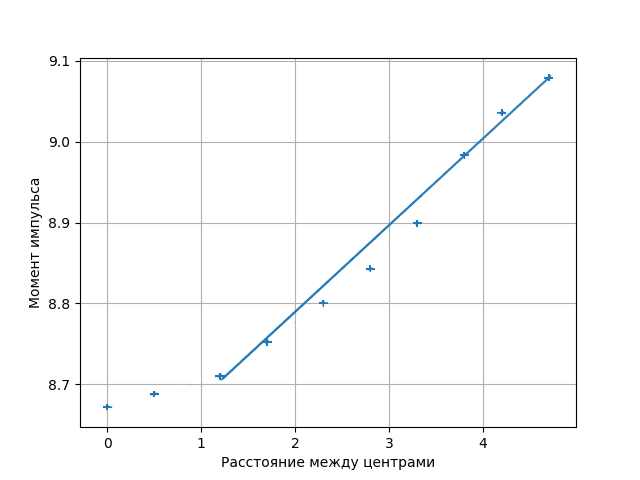
\includegraphics[width=0.75\linewidth]{Figure_1.png}
    \caption{Зависимость $I$ от $2h$}
\end{figure}

\noindent
То, что полученные точки плохо ложатся на прямую можно обьяснить тем, что в ходе эксперимента ось вращения не была неподвижной, так как закручивали нижнюю платформу, что крайне затруднительно сделать не вызвав ее раскачиваний. Чтобы избежать такого отклонения следует закручивать верхнюю платформу.

\section*{Вывод}

\noindent
С помощью трифилярного подвеса можно достаточно точно измерить момент инерции тела, а так же экспериментально подтвердить аддитивность моментов инерции и, предположительно, формулу Гюйгенса-Штейнера, но для этого требуется проводить вычисления с наименьшими приданными раскачиваниями нижней платформы. 

\end{document}
